\documentclass[conference]{IEEEtran}
\IEEEoverridecommandlockouts
\usepackage{cite}
\usepackage{amsmath,amssymb,amsfonts}
\usepackage{algorithmic}
\usepackage{graphicx}
\usepackage{textcomp}
\usepackage{xcolor}
\usepackage{array}
\usepackage{url}

\renewcommand{\algorithmicrequire}{\textbf{Require:}}

\makeatletter
\newcommand{\linebreakand}{%
  \end{@IEEEauthorhalign}
  \hfill\mbox{}\par
  \mbox{}\hfill\begin{@IEEEauthorhalign}
}
\makeatother


\begin{document}

\title{EdgeInterview: A Privacy-Preserving, On-Device\\ Multi-Modal AI Interview Coach}

\author{\IEEEauthorblockN{Mayank}
\IEEEauthorblockA{\textit{School of Computer Science and Engineering} \\
\textit{Vellore Institute of Technology}\\
Vellore, India \\
mayank.2023a@vitstudent.ac.in}
\and
\IEEEauthorblockN{Yashwin}
\IEEEauthorblockA{\textit{School of Computer Science and Engineering} \\
\textit{Vellore Institute of Technology}\\
Vellore, India \\
yashwin.2023@vitstudent.ac.in}
\linebreakand
\IEEEauthorblockN{Tanisi Narwal}
\IEEEauthorblockA{\textit{School of Computer Science and Engineering} \\
\textit{Vellore Institute of Technology}\\
Vellore, India \\
tanisi.narwal2023@vitstudent.ac.in}
\and
\IEEEauthorblockN{Banupriya R}
\IEEEauthorblockA{\textit{School of Computer Science and Engineering} \\
\textit{Vellore Institute of Technology}\\
Vellore, India \\
banupriya.r@vit.ac.in}
}

\maketitle

\begin{abstract}
Mock interview platforms are used by students to prepare for job interviews. They either find a mentor who is willing to conduct a mock interview with them, or use online AI interview platforms which require them to upload their resume and stream their voice and video to a third party server. This paper introduces Edge Interview, a mock interview platform which can be run on the candidate's laptop offline. It conducts a spoken, turn-based conversation, asks questions based on the candidate's resume and target role, provides follow-ups if the answer is too shallow, and generates a question-by-question report after the interview. The questions and answer grading are powered by a 4-billion-parameter language model hosted locally via Ollama. However, due to the unreliability of a model of this size, the control of the interview is not entirely delegated to it. Instead, all proposals made by the model are validated by a deterministic backend controller which manages follow-up budgets, topic transitions, and interview conclusion. The turn-taking logic is based on a self-calibrating energy-based voice activity detector with an independent hard timeout. The scoring is deferred to the end of the session, and the score is stored once via an atomic database claim. An optional camera module provides presentation feedback relative to the candidate's own baseline, and avoids inferring emotions or personality following the literature on bias in automated interviews. The platform was able to successfully complete all 23 test sessions without any hangs, and the use of the camera module did not have any measurable impact on turn latency.
\end{abstract}

\begin{IEEEkeywords}
mock interview, local language model, voice activity detection, deterministic control, fairness in AI, offline processing, presentation feedback
\end{IEEEkeywords}

\section{Introduction}
Before job placements, students can gain a lot of value from mock interviews. However, it can be difficult to find a mentor or senior who is willing to conduct a mock interview with them. Online AI interview tools address the availability of mock interviews, but they introduce some other issues. Firstly, they require candidates to share their personal information (resume, voice, and often live video) with a third party server. Secondly, some of these tools score candidates based on the signals from their facial video. The psychological evidence does not support the inference of internal states from facial movement~\cite{barrett2019}. Furthermore, there is a growing regulatory trend to restrict the use of such analysis in hiring and education~\cite{euaiact,illinois,nyc144}.

Our goal was to explore the feasibility of a mock interview tool that would feel more like a conversation rather than a fixed quiz, while keeping all candidate information on the candidate's laptop. With the advent of small language models, this is now possible with consumer-grade hardware. However, these models come with their own reliability issues. During the development of the system, we realized that the 4B-parameter model could sometimes terminate the interview after a few minutes, continuously ask follow-ups on the same point, or fail to output some fields in the structured output. Although we could mitigate some of these issues via prompt engineering, we were not able to eliminate them completely.

Therefore, we decided to restrict the control of the model. The large language model (LLM) is used to generate questions and grade the content, while the deterministic controller manages all decisions that affect the interview flow. This is in the spirit of a deterministic control plane around an LLM agent~\cite{madatha2026}. In this paper, we make the following main contributions:
\begin{itemize}
\item A fully offline, voice-based mock interview pipeline that adapts questions based on the candidate's resume and answers, using only local models.
\item A design for the controller, where a small local LLM suggests the next action and a rule-based component either accepts or overrides it, along with the failure cases which led to this design.
\item A non-stalling turn-taking logic, which combines a self-calibrating voice activity detector (VAD) with an independent timeout, and uses a single state variable to gate both the microphone and speaker.
\item A deferred, idempotent evaluation phase, which ensures that the stored score is never modified when re-opening an interview.
\item An optional camera-based feedback module, which provides description of behaviour relative to the candidate's own baseline, and is designed following the literature on bias in automated video interviews~\cite{booth2023,fabris2023}.
\end{itemize}

The rest of the paper is organized as follows. Section~\ref{sec:related} presents related work. Section~\ref{sec:arch} describes the system architecture. Section~\ref{sec:method} details each phase in the pipeline. Section~\ref{sec:impl} explains the implementation. Section~\ref{sec:results} presents the results from our test sessions. Section~\ref{sec:limits} discusses the limitations. Finally, we conclude the paper.

\section{Related Work}\label{sec:related}

\begin{figure*}[t]
\centering
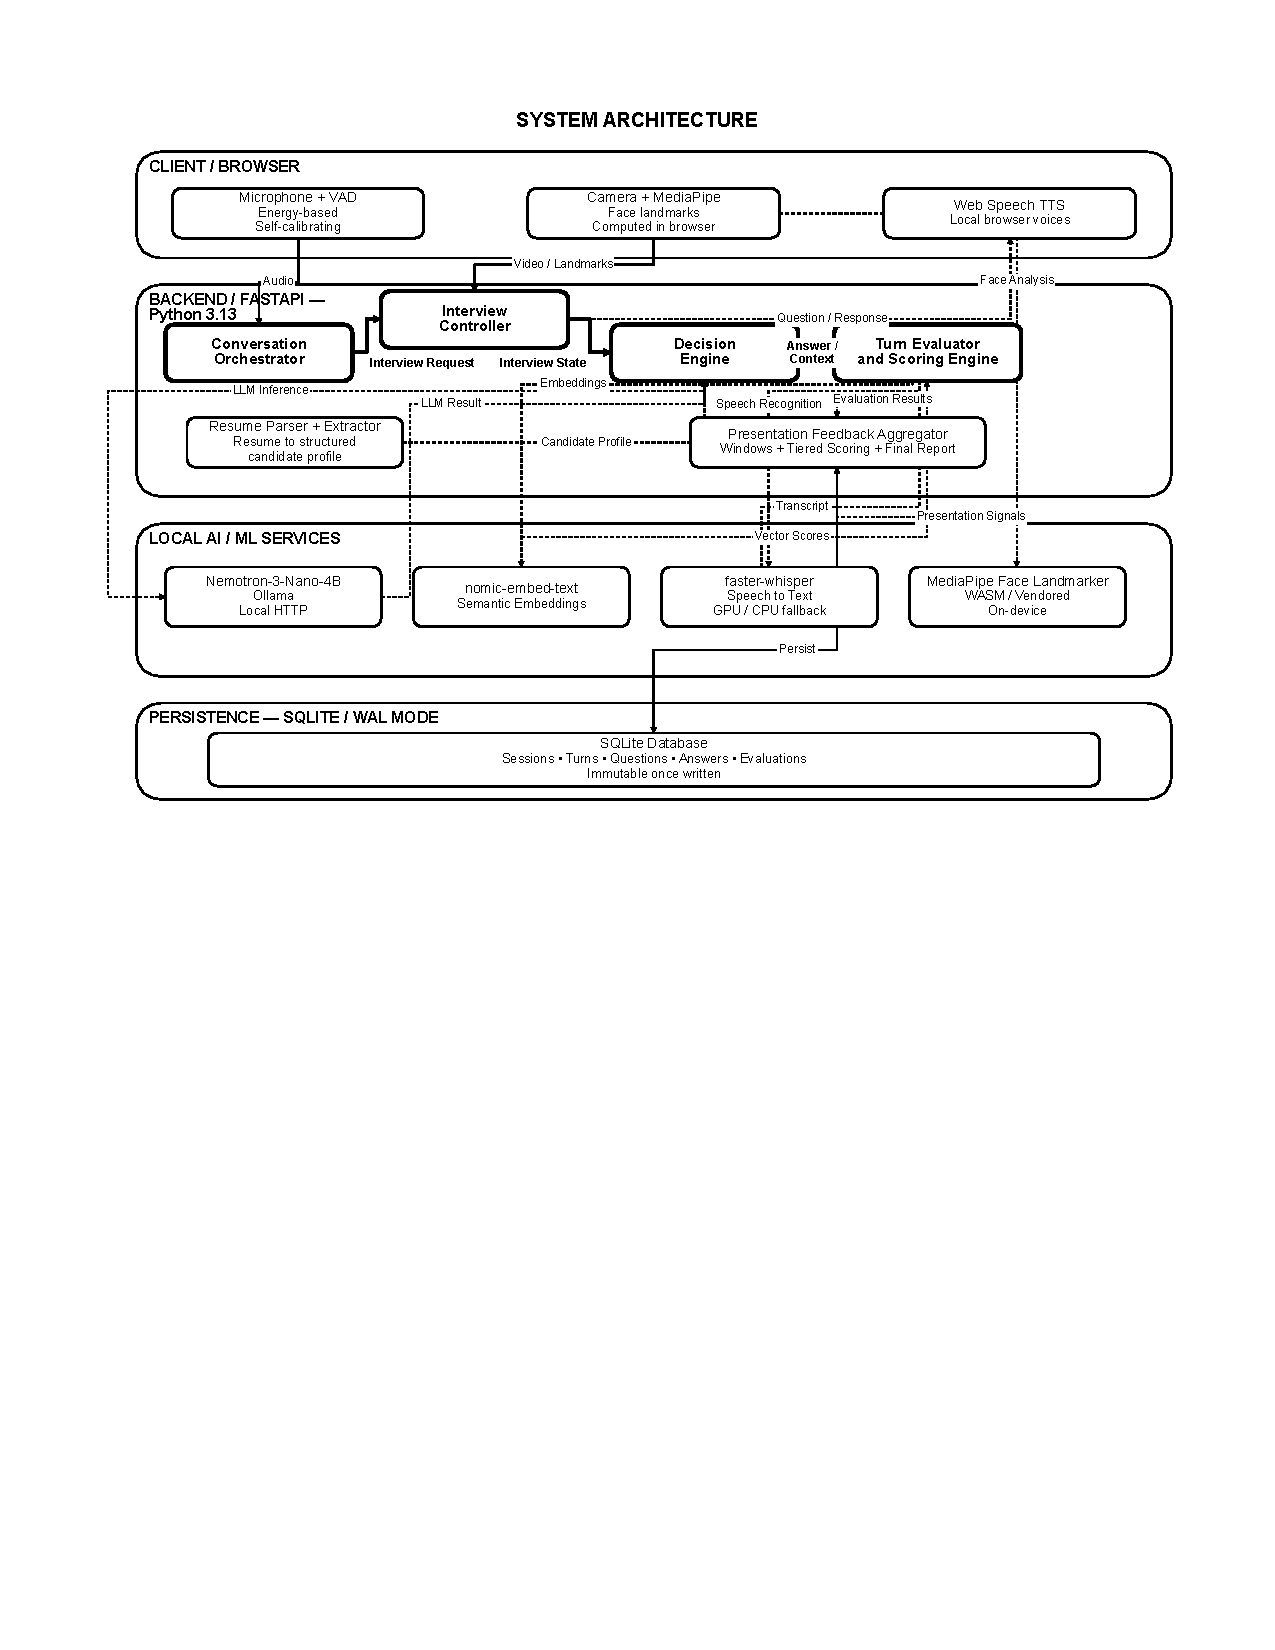
\includegraphics{fig1.pdf}
\caption{System architecture. Client browser, FastAPI backend, local AI services, and SQLite store are all running on the candidate's laptop. No component makes external network calls.}
\label{fig:arch}
\end{figure*}


\subsection{Automated Interview Coaching}
Automated interview practice has been a subject of research for more than a decade. MACH~\cite{hoque2013} used a virtual agent that perceived user's speech and facial expression and provided feedback after the session. Naim et al.~\cite{naim2018} predicted human-rated interview performance based on prosodic, lexical, and facial features. These studies demonstrated the benefits of automated feedback for improving performance. However, they either rely on cloud processing or controlled lab environments. In particular, the second group of work uses facial signals as predictors of performance, which we chose to avoid.

\subsection{Speech, Vision, and Language Components}
Whisper~\cite{radford2022} enabled practical, local speech recognition. Even the smallest model is sufficient for handling clear English speech for interview answers. MediaPipe~\cite{lugaresi2019} provides on-device, real-time face and hand landmark tracking in a browser. On the language side, state-space models like Mamba~\cite{gu2023} reduce the cost of generating long sequences, which can help a hybrid model like Nemotron-3-Nano-4B to respond within the turn. We use Nomic Embed~\cite{nussbaum2024}, which is an openly trained text embedder that can be run locally, in the spirit of retrieval-augmented generation~\cite{lewis2020}, for resume retrieval. For classical voice activity detection, statistical models of speech and noise are often used~\cite{sohn1999}. We use a simpler energy-threshold-based approach, which is cheap to run in the browser and easy to calibrate per session.

\subsection{Reliability of Small LLMs}
Schema-constrained decoding is a common technique used to obtain structured output from an LLM. Beurer-Kellner et al.~\cite{beurer2024} explore the interaction between the constraints and the LLM's token distribution. This helped us understand one of our bugs, where optional fields in our schema were being silently omitted. More generally, the idea of surrounding an LLM agent with a deterministic controller that validates all actions~\cite{madatha2026} is used in our backend.

\subsection{Fairness and Regulation}
Barrett et al.~\cite{barrett2019} reviewed the evidence on facial expressions and concluded that they are not a reliable indicator of emotional state. Booth et al.~\cite{booth2023} surveyed bias in automated video interviews, identifying various features, such as gaze patterns and amount of movement, that can vary across demographic groups. Fabris et al.~\cite{fabris2023} reviewed fairness in algorithmic hiring in general. There is a growing regulatory trend in this area. For example, the EU AI Act prohibits emotion recognition in the workplace and education~\cite{euaiact}. Illinois requires notice and consent for AI analysis of interview video~\cite{illinois}. New York City requires bias audits of automated employment decision tools~\cite{nyc144}. These works directly influenced the design of the presentation feedback module, which is described in Section~\ref{sec:present}.

\begin{table}[t]
\caption{Comparison With Common Practice Options}
\label{tab:compare}
\centering
\footnotesize
\renewcommand{\arraystretch}{1.3}
\begin{tabular}{|l|c|c|c|}
\hline
\textbf{Property} & \textbf{Human} & \textbf{Cloud AI} & \textbf{Ours} \\
\hline
Available on demand & No & Yes & Yes \\
Data on device & Yes & No & Yes \\
Adaptive follow-up questions & Yes & Varies & Yes \\
Bounded LLM authority & -- & Rarely & Yes \\
No emotion inference from video & Yes & Varies & Yes \\
Internet or paid service required & No & Yes & No \\
\hline
\end{tabular}
\end{table}

In Table~\ref{tab:compare}, we compare our approach with the two common alternatives. To our knowledge, there is no openly available system that can run offline, be adaptive in the conversation, have deterministic flow control, and feature an inference-free video module.

\section{System Architecture}\label{sec:arch}
Our system is structured into four layers, as shown in Fig.~\ref{fig:arch}. All of these layers run on the same machine.

\textit{Client (browser).} The client is a simple HTML, CSS, and JavaScript, which is served from the backend. It captures the microphone audio, runs the VAD and the turn-taking state machine, and speaks the questions using the locally installed voices in the browser. If the candidate opts in, MediaPipe is run in the browser. Only the landmark coordinates are sent, so the raw video never leaves the page.

\textit{Backend.} This is a FastAPI service written in Python 3.13. It hosts six components. Conversation Orchestrator receives audio and requests. Interview Controller manages the state of the interview and has the final say on the next action. Decision Engine generates prompts and parses the proposals from the LLM. Turn Evaluator and Scoring Engine grades the answers. resume Parser parses the uploaded PDF to generate a structured candidate profile. Presentation Feedback Aggregator aggregates the landmark streams into windowed metrics and a final summary.

\textit{Local AI services.} We use Ollama to host Nemotron-3-Nano-4B for question generation and grading. We also use nomic-embed-text for embeddings, which is hosted over a local HTTP port. For speech recognition, we use faster-whisper with the tiny model on the GPU, falling back to the CPU if there is no GPU. For face landmarker, we vendor MediaPipe as WebAssembly, so it can run without a network connection.

\textit{Persistence.} We use SQLite with write-ahead-logging (WAL) mode to store sessions, turns, questions, answers, and evaluations. We treat evaluations as immutable after writing them.

\section{Methodology}\label{sec:method}

\subsection{resume Ingestion and Topic Planning}
We read the uploaded PDF using PyMuPDF. We use heuristic rules to split the text into various sections, such as education, projects, experience, and skills. We embed each section using nomic-embed-text and store them. At the beginning of the interview, we rank the sections based on their similarity to the stated target role. This ranking serves as the topic plan for the controller. The LLM drafts the opening question based on the top-ranked section, which is then validated by the controller, like any other proposal.

\subsection{Voice Turn-Taking}
This is the part of the system that we had the most failures with during development. All the failures manifested in the same way to the user. The interview appeared to freeze after the user stopped speaking. Our final design consists of the following three parts.

\textit{Calibration.} For the first two seconds of the session, the client measures the root-mean-square (RMS) energy of the raw microphone signal. We take the mean of the RMS energy as the noise floor
\begin{equation}
E_0 = \frac{1}{N}\sum_{n=1}^{N} e_n,
\label{eq:floor}
\end{equation}
where $e_n$ is the RMS energy of frame $n$ and $N$ is the number of frames in the calibration window. We consider a frame to be speech if its energy is greater than the noise floor in (\ref{eq:floor}) plus a margin. That is, if
\begin{equation}
e_n > E_0 + \delta,
\label{eq:speech}
\end{equation}
where $\delta$ is a fixed margin. By calibrating per session, the same code can be used for a laptop microphone in a quiet room, or a headset in a noisy hostel.

\textit{End of utterance.} We consider the answer to be over after roughly 1.6~s of no frame satisfying (\ref{eq:speech}). We allow one noisy frame in the silence timer, as we found that a single stray spike can reset the silence timer indefinitely in a noisy room. We use the raw signal for detection, rather than the amplified signal displayed in the level meter on the screen. Using the display signal caused one of our hangs.

\textit{Hard timeout.} Independently of the VAD, we use a 5~s timer to advance the state machine if the candidate never starts speaking. This ensures progress, even if the VAD fails in an unexpected way.

This is coordinated by the state machine shown in Fig.~\ref{fig:fsm}. We use a single state variable to gate both devices. We only record the microphone in WAITING\_FOR\_USER and USER\_SPEAKING states. We only play speech in the BOT\_SPEAKING state. This ensures that the system cannot transcribe its own voice as the candidate's answer.

\begin{figure}[t]
\centering
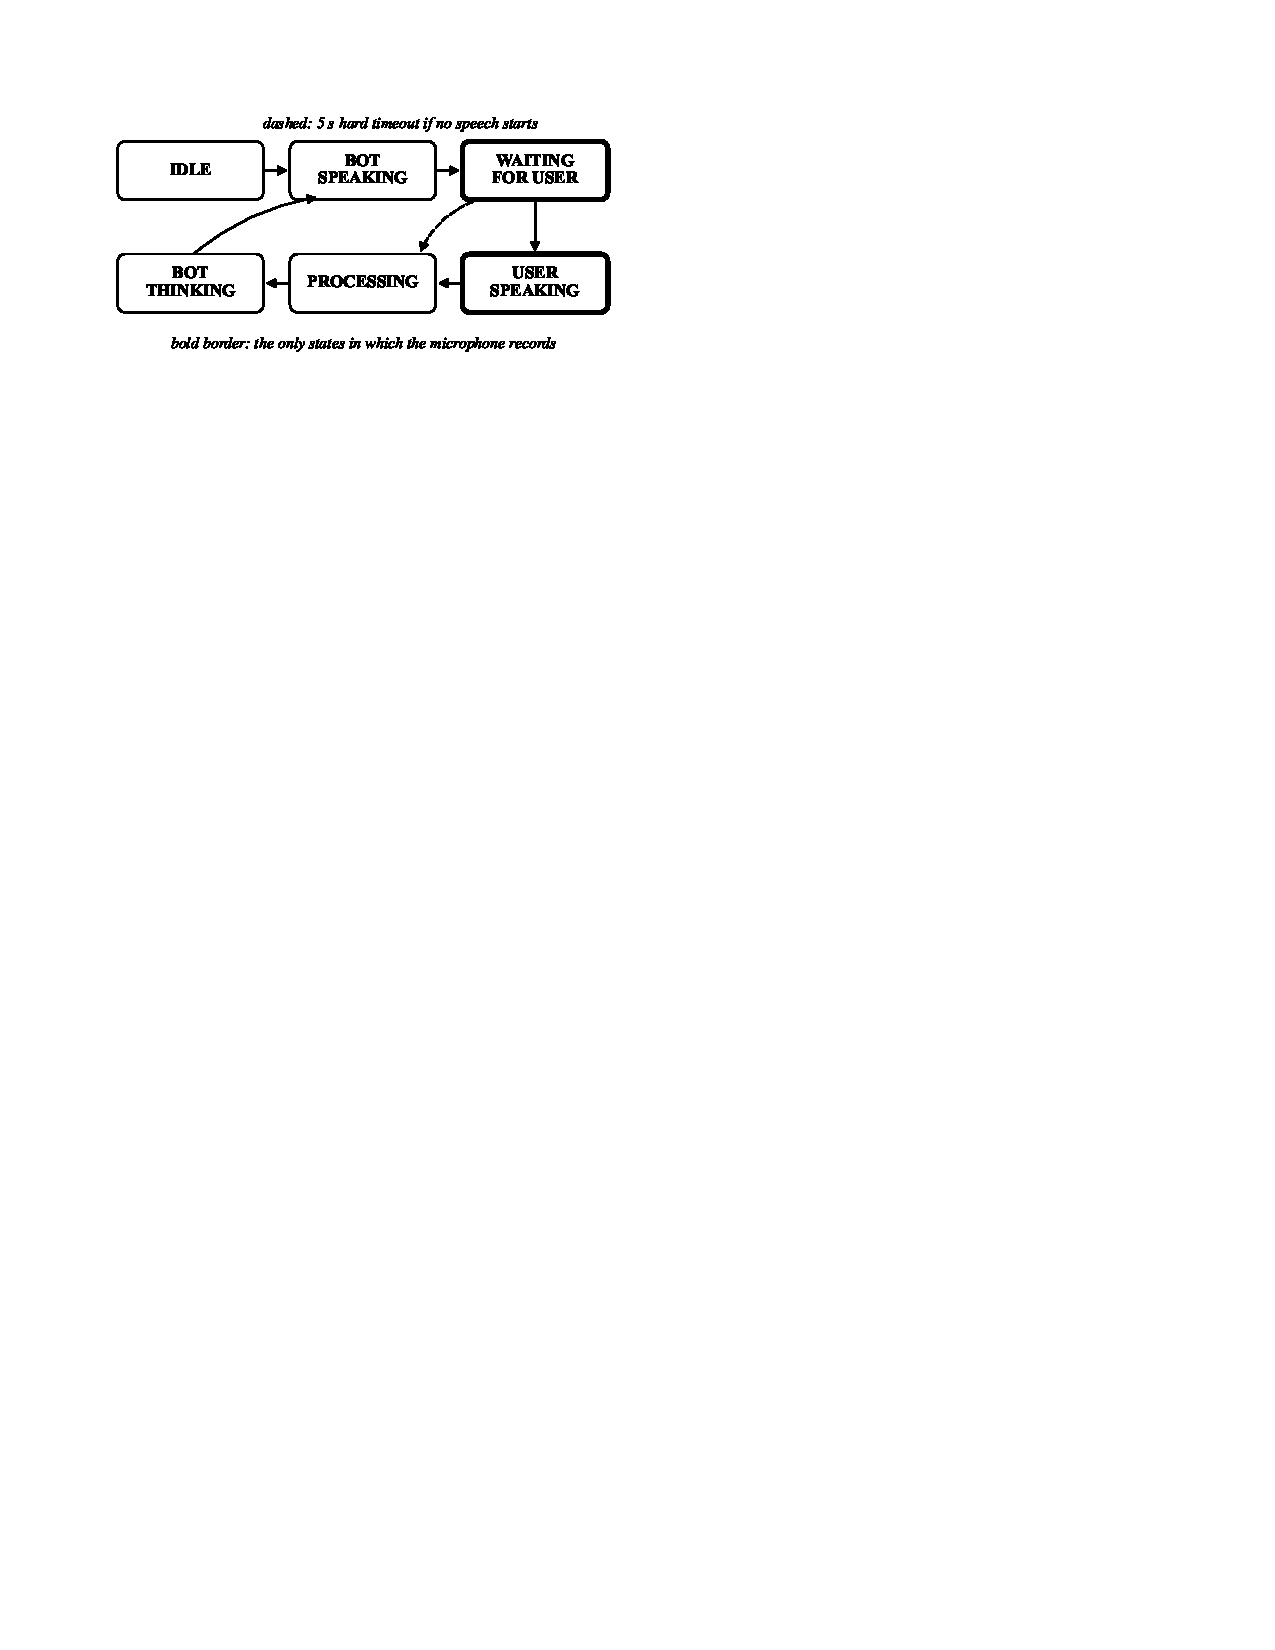
\includegraphics{fig2.pdf}
\caption{Client-side turn-taking state machine. Dashed transition is the hard timeout.}
\label{fig:fsm}
\end{figure}

\begin{figure}[t]
\begin{algorithmic}[1]
\REQUIRE proposal $(a,q,u)$; $f$ used follow-ups on current topic; $T_r$ time remaining
\REQUIRE limits $F_{\max}$, $\tau$, $T_{\min}$
\IF{$a = \textsc{Conclude}$ \textbf{and} $T_r > T_{\min}$}
\STATE $a \leftarrow \textsc{NextTopic}$
\ENDIF
\IF{$a = \textsc{FollowUp}$ \textbf{and} $(f \geq F_{\max}$ \textbf{or} $u \geq \tau)$}
\STATE $a \leftarrow \textsc{NextTopic}$
\ENDIF
\IF{$a = \textsc{NextTopic}$ \textbf{and} topic plan is empty}
\STATE $a \leftarrow \textsc{Conclude}$
\ENDIF
\IF{$a$ was changed}
\STATE $q \leftarrow$ planned question for the resulting action
\ENDIF
\RETURN $(a,q)$
\end{algorithmic}
\caption{Controller decision rules applied in each turn.}
\label{fig:rules}
\end{figure}

\subsection{Deterministic Interview Controller}
The session runs in an asynchronous loop. For each turn, the backend transcribes the answer, updates the interview state (topics covered, used follow-ups on the current topic, time remaining), requests a proposal from the LLM, and passes the proposal to the controller. The LLM responds with a fixed JavaScript Object Notation (JSON) schema. The schema includes the understanding score for the latest answer, the proposed action (FOLLOW\_UP, NEXT\_TOPIC, or CONCLUDE), and the question text. All fields in the schema are marked as required. When we had optional fields, the model often omitted them, and we ended up with incomplete proposals for downstream code~\cite{beurer2024}.

We then apply the rules shown in Fig.~\ref{fig:rules}. We only allow follow-up if we still have budget on the current topic and the answer is too shallow. We only accept the request to conclude if there is little time remaining. If the controller rejects the proposal, we replace it with the next question from the topic plan. This allows the model to influence the conversation, but not break the structure.

We end the session when we run out of time budget, or when the topic plan is exhausted, or if the candidate ends the session. We have a Quick-practice mode where we skip the LLM proposal altogether and ask a fixed set of questions derived from the resume. This can help with latency for short drills.

\subsection{Deferred and Idempotent Evaluation}
If we were to grade the answers during the conversation, this would require us to call the model for each turn. Therefore, we defer all the scoring until after the session is closed. During the evaluation job, we first claim the session with a single conditional update.
\begin{center}
\small
\begin{tabular}{l}
\texttt{UPDATE interviews SET evaluated=1}\\
\texttt{\ \ \ \ WHERE id=? AND evaluated=0}
\end{tabular}
\end{center}
We only proceed if exactly one row was updated. If no row was updated, then either another worker has already claimed the session or it has already been scored. In this case, we do not re-run anything. Thus, when we re-open an old interview, we only read the stored report. There is no change to the score.

For each answer, we assign three scores on a scale of 0--10. The content score $S_c$ is provided by the LLM. It grades the answer based on a rubric, which includes the relevance, depth, use of concrete examples, and technical correctness of the answer. We grade the answers in batches, along with a holistic pass over the entire transcript. We check that each returned score is on the 0--10 scale before storing it. The delivery score $S_d$ is calculated in plain Python based on the transcript. This includes the filler-word ratio, variation in sentence length, penalties for answers that are too short or too long, and detection of structured answers like the situation, task, action, result (STAR) pattern. There is no model call involved in this. The overall score is
\begin{equation}
S = 0.65\,S_c + 0.35\,S_d.
\label{eq:score}
\end{equation}
We use a higher weight for the content in (\ref{eq:score}), as the candidate's answer is more important than the fluency in a technical mock interview.

\subsection{Presentation Feedback}\label{sec:present}
The camera module is disabled by default. We only enable it after an explicit consent screen, following the notice-and-consent model from~\cite{illinois}. When enabled, we compute five metrics from the landmark stream in fixed time windows. These include eye-contact ratio, head-pose stability, blink rate, postural sway, and gesture frequency. For each metric $m$, we use the first ten seconds of the session to establish a personal baseline $b_m$. For each subsequent window, we report the deviation $\Delta_m$ as
\begin{equation}
\Delta_m = x_m - b_m.
\label{eq:dev}
\end{equation}
We only report the deviations from (\ref{eq:dev}). We do not compare any metric to an external ``ideal'' value. For gaze direction and amount of movement, we report the numbers as plain numbers. We do not use any positive or negative framing, as both can vary across demographic groups~\cite{booth2023}. We do not perform any emotion classification. We do not infer personality or employability~\cite{barrett2019,euaiact}. We do not combine the output of this module with the interview score.

\section{Implementation}\label{sec:impl}

\begin{table}[t]
\caption{Software Stack}
\label{tab:stack}
\centering
\footnotesize
\renewcommand{\arraystretch}{1.3}
\begin{tabular}{|l|l|}
\hline
\textbf{Function} & \textbf{Component} \\
\hline
Web server & FastAPI with uvicorn (Python 3.13) \\
Language model & Nemotron-3-Nano-4B via Ollama \\
Embeddings & nomic-embed-text v1.5 via Ollama \\
Speech to text & faster-whisper (tiny) \\
Text to speech & Browser voices (local) \\
Landmarks & MediaPipe Face Mesh and Hands \\
PDF parsing & PyMuPDF \\
Storage & SQLite (WAL mode) \\
\hline
\end{tabular}
\end{table}

\begin{table}[t]
\caption{Statistics From 23 Test Sessions}
\label{tab:stats}
\centering
\footnotesize
\renewcommand{\arraystretch}{1.3}
\begin{tabular}{|l|c|}
\hline
\textbf{Measure} & \textbf{Value} \\
\hline
Completed sessions & 23 \\
Median questions per session & 12 \\
Median session length & 18 min \\
Sessions that used the full follow-up budget & 61\% \\
Sessions where the hard timeout fired & 4 of 23 \\
Sessions that hung or crashed & 0 \\
\hline
\end{tabular}
\end{table}

The main software components are listed in Table~\ref{tab:stack}. The backend is written in Python 3.13 and consists of around 3,200 lines of Python across 18 modules. The frontend is written in HTML, CSS, and JavaScript. It consists of around 2,100 lines across six files. We do not use any bundler or framework. For development and all the measurements in this paper, we used a laptop with an NVIDIA RTX 4060 Laptop GPU (8~GB). The system also runs on CPU only with higher latency.

We used a combination of four techniques for testing. For each change in the frontend, we checked with \texttt{node --check}. We also had a small script that cross-checked every element ID used in JavaScript against the HTML. We write the video windowing, calibration, and tiered scoring logic as pure functions. We have 81 assertions that we run directly in Node. We have standalone diagnostic pages that exercise the camera pipeline, inference timing, and report generation in isolation. This allows us to narrow down a failure to a specific subsystem. Finally, we drove the full application in a real Chrome browser against the live backend. This hardware-in-the-loop testing allowed us to find all three VAD defects described in Section~\ref{sec:results}. None of these were present in synthetic tests or code review.

\section{Results}\label{sec:results}
Since there is no public dataset for this kind of system, we report the data from the system's logs during development and testing. This should be viewed as an engineering evaluation, rather than a user study.

\subsection{Session Behaviour}
Table~\ref{tab:stats} shows the summary of 23 complete interview sessions, which we ran on the development machine. All the sessions successfully completed without any hangs or crashes. The follow-up budget was used up in 61\% of the sessions. This indicates that the adaptive follow-up path is regularly exercised and not a rare branch. We had the hard timeout fire at least once in 4 out of the 23 sessions. We originally added the timeout as a safety net, but it is actually needed in normal use based on these results.

\begin{figure}[t]
\centering
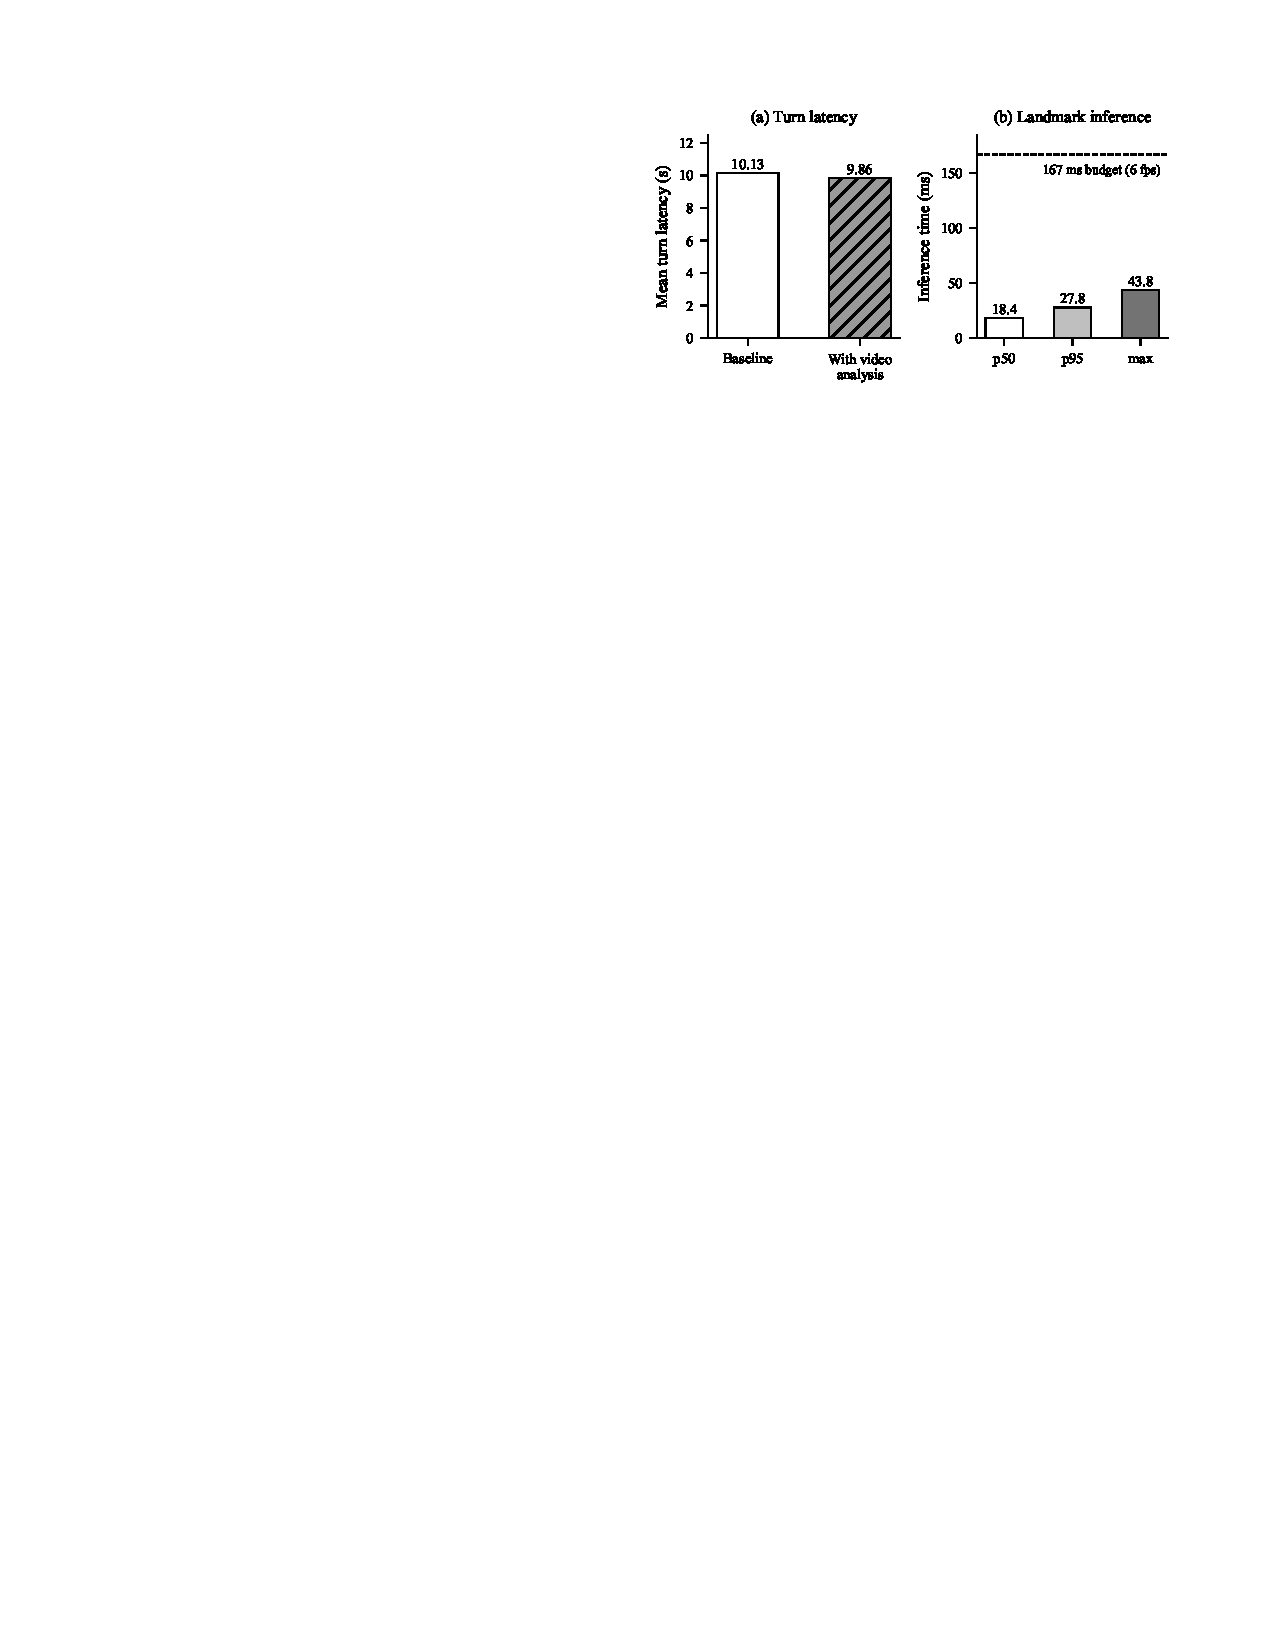
\includegraphics{fig4.pdf}
\caption{(a) Mean turn latency with and without video analysis. (b) Face-landmark inference time on an RTX 4060 Laptop GPU.}
\label{fig:latency}
\end{figure}

\subsection{Adaptive Follow-up Example}
In one of our recorded sessions, the candidate provided a vague answer to a system design question. The LLM proposed a follow-up asking for a concrete example. The controller allowed this follow-up, as there was still budget remaining and the understanding score was low. The second answer was significantly more specific, and the understanding score increased above the threshold $\tau$. Therefore, the controller moved on to the next topic instead of allowing a third follow-up. A fixed question list cannot do this. An unconstrained model may not reliably stop at this point.

\subsection{Latency}
Fig.~\ref{fig:latency}(a) shows the comparison of the mean turn latency with and without the camera module running. The difference is 0.27~s, which is within the run-to-run noise. This is expected, as the landmark inference is running in the browser. Only small coordinate arrays are sent to the backend. Fig.~\ref{fig:latency}(b) shows the face-landmark inference time. The median is 18.4~ms. The 95th percentile is 27.8~ms. The worst case is 43.8~ms. This is well within the 167~ms available per frame at 6 frames per second. Most of the turn time is consumed by language model generation and speech. This is where we should focus our future efforts for optimization.

\subsection{Defects Found During Development}
During the development, we maintained a log of defects. Fig.~\ref{fig:defects} shows a representative sample of 13 defects, grouped into categories. The largest category was LLM reliability issues. This included dropped schema fields, occasionally returning scores on a 0--1 scale instead of 0--10, and trying to conclude the interview prematurely. The most difficult issues to diagnose were the voice and VAD issues. We had three different root causes that led to the same symptom. This included missing an independent timeout, taking a decision based on the amplified display signal, and resetting the silence timer due to a single noisy frame. In Table~\ref{tab:failures}, we map each failure to the design element which now prevents it.

\begin{figure}[t]
\centering
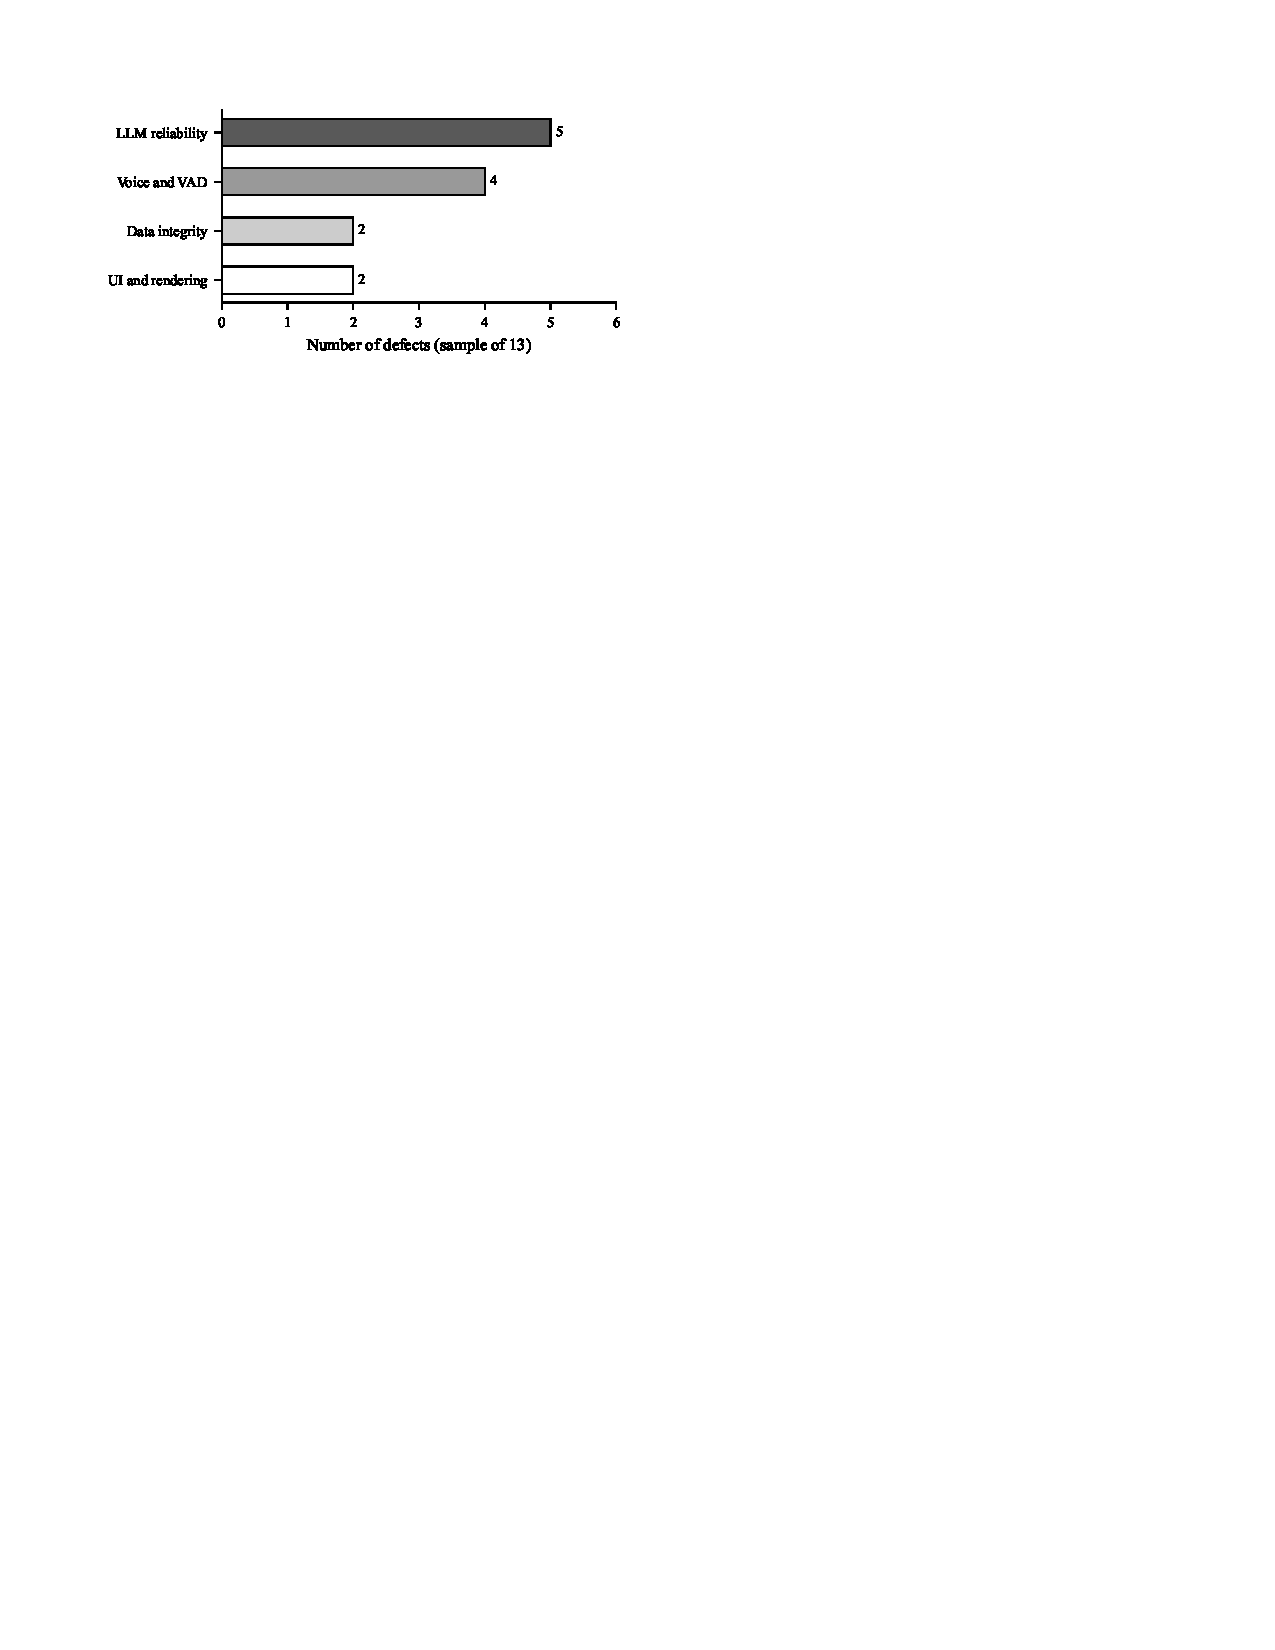
\includegraphics{fig5.pdf}
\caption{Defect categories in a sample of 13 defects logged during development.}
\label{fig:defects}
\end{figure}

\begin{table}[t]
\caption{Observed Failures and Design Responses}
\label{tab:failures}
\centering
\footnotesize
\renewcommand{\arraystretch}{1.3}
\begin{tabular}{|p{104pt}|p{104pt}|}
\hline
\textbf{Failure} & \textbf{Design response} \\
\hline
Interview appears to freeze after the answer & Independent hard timeout; VAD on raw signal; silence timer tolerates one noisy frame \\
\hline
System hears its own voice & One state variable gates microphone and speaker \\
\hline
LLM drops output fields & All schema fields required \\
\hline
LLM ends interview too early & Conclude accepted only when little time remains \\
\hline
Scores on wrong scale & Range check before storage \\
\hline
Score changes on reopening & Atomic claim; evaluations immutable \\
\hline
\end{tabular}
\end{table}

\section{Limitations}\label{sec:limits}
In this paper, we present a small-scale evaluation. All 23 sessions were run on the same machine by the development team. Therefore, these results indicate that the system works reliably. However, they do not indicate that the system improves the performance in the interview. A proper user study with external participants is the most important next step. Our system currently only supports English. We would need to evaluate both the speech model and the prompts for other languages. Content grading is still dependent on a 4B model. Although the controller limits the authority of the model on the flow of the interview, we have not stress-tested the quality of its judgements for unusual or adversarial answers. We do not have speaker diarisation, so the system assumes a single speaker. Our resume parsing is heuristic. We have only checked it with a small number of formats. Finally, we write the deterministic scoring code on the backend as pure functions, but we do not have an automated test suite for it yet.

\section{Conclusion and Future Work}
We presented Edge Interview, which is an offline mock interview system. It conducts an adaptive spoken conversation, grades the answers, and reports the results without sending any candidate data off the device. The main takeaway from building this system is that a small local language model can be fast and private enough to be useful in a live conversation. However, we should not trust the model to make control decisions on its own. By delegating those decisions to a deterministic controller, deferring and freezing the evaluation, and designing the turn-taking in a way that always makes progress, we turned an unreliable prototype into a system that was able to successfully complete all the test sessions. This caution is also reflected in our camera module, which provides description of behaviour relative to the candidate's own baseline, and does not make any claims about emotion or personality.

In future work we plan to add a pytest suite for the controller and scoring modules, run a user study with real candidates to test whether the follow-ups and presentation feedback are perceived as fair and useful, extend the system to other languages, and package it as a single installer so that students do not need to set up Python and Ollama by hand.

\section*{Acknowledgment}
The authors thank Dr. Banupriya R for guidance throughout this project and the School of Computer Science and Engineering for its support.

\begin{thebibliography}{00}
\bibitem{barrett2019} L.~F. Barrett, R.~Adolphs, S.~Marsella, A.~M. Martinez, and S.~D. Pollak, ``Emotional expressions reconsidered: Challenges to inferring emotion from human facial movements,'' \textit{Psychological Science in the Public Interest}, vol.~20, no.~1, pp.~1--68, 2019.
\bibitem{euaiact} European Union, ``Regulation (EU) 2024/1689 (Artificial Intelligence Act), Article 5(1)(f),'' Official Journal of the European Union, 2024.
\bibitem{illinois} Illinois General Assembly, ``Artificial intelligence video interview act, 820 ILCS 42,'' 2020.
\bibitem{nyc144} New York City Council, ``Local law 144 of 2021: Automated employment decision tools,'' 2021.
\bibitem{madatha2026} P.~Madatha, ``A deterministic control plane for LLM coding agents,'' arXiv preprint arXiv:2606.26924, 2026.
\bibitem{booth2023} B.~M. Booth, L.~Hickman, S.~K. Subburaj, L.~Tay, S.~E. Woo, and S.~K. D'Mello, ``Integrating psychometrics and computing perspectives on bias and fairness in affective computing: A case study of automated video interviews,'' arXiv preprint arXiv:2305.02629, 2023.
\bibitem{fabris2023} A.~Fabris, N.~Baranowska, M.~J. Dennis, D.~Graus, P.~Hacker, J.~Saldivar, F.~Z. Borgesius, and A.~J. Biega, ``Fairness and bias in algorithmic hiring: A multidisciplinary survey,'' arXiv preprint arXiv:2309.13933, 2023.
\bibitem{hoque2013} M.~E. Hoque, M.~Courgeon, J.-C. Martin, B.~Mutlu, and R.~W. Picard, ``MACH: My automated conversation coach,'' in \textit{Proc. ACM Int. Joint Conf. Pervasive and Ubiquitous Computing (UbiComp)}, 2013, pp.~697--706.
\bibitem{naim2018} I.~Naim, M.~I. Tanveer, D.~Gildea, and M.~E. Hoque, ``Automated analysis and prediction of job interview performance,'' \textit{IEEE Transactions on Affective Computing}, vol.~9, no.~2, pp.~191--204, 2018.
\bibitem{radford2022} A.~Radford, J.~W. Kim, T.~Xu, G.~Brockman, C.~McLeavey, and I.~Sutskever, ``Robust speech recognition via large-scale weak supervision,'' arXiv preprint arXiv:2212.04356, 2022.
\bibitem{lugaresi2019} C.~Lugaresi, J.~Tang, H.~Nash, C.~McClanahan, E.~Uboweja, M.~Hays, F.~Zhang, C.-L. Chang, M.~G. Yong, J.~Lee, W.-T. Chang, W.~Hua, M.~Georg, and M.~Grundmann, ``MediaPipe: A framework for building perception pipelines,'' arXiv preprint arXiv:1906.08172, 2019.
\bibitem{gu2023} A.~Gu and T.~Dao, ``Mamba: Linear-time sequence modeling with selective state spaces,'' arXiv preprint arXiv:2312.00752, 2023.
\bibitem{nussbaum2024} Z.~Nussbaum, J.~X. Morris, B.~Duderstadt, and A.~Mulyar, ``Nomic embed: Training a reproducible long context text embedder,'' arXiv preprint arXiv:2402.01613, 2024.
\bibitem{lewis2020} P.~Lewis, E.~Perez, A.~Piktus, F.~Petroni, V.~Karpukhin, N.~Goyal, H.~K\"uttler, M.~Lewis, W.~tau Yih, T.~Rockt\"aschel, S.~Riedel, and D.~Kiela, ``Retrieval-augmented generation for knowledge-intensive NLP tasks,'' in \textit{Advances in Neural Information Processing Systems}, vol.~33, 2020, pp.~9459--9474.
\bibitem{sohn1999} J.~Sohn, N.~S. Kim, and W.~Sung, ``A statistical model-based voice activity detection,'' \textit{IEEE Signal Processing Letters}, vol.~6, no.~1, pp.~1--3, 1999.
\bibitem{beurer2024} L.~Beurer-Kellner, M.~Fischer, and M.~Vechev, ``Guiding LLMs the right way: Fast, non-invasive constrained generation,'' arXiv preprint arXiv:2403.06988, 2024.
\end{thebibliography}

\end{document}
